\documentclass{article}
\usepackage{graphicx} % Required for inserting images
\usepackage{hyperref} % For url links
\usepackage{amsmath} % For math eqns
\usepackage{MnSymbol}
\usepackage{xcolor} % For coloring text (used for links)
\usepackage{csquotes}
\usepackage[style=ieee, backend=biber]{biblatex} 
\usepackage{ulem}   % For strikethrough effect
\DeclareFieldFormat{sentencecase}{#1}
\addbibresource{our_bib.bib}


\title{Reinforcement Learning\\ \large{Final Report}}
\author{Mathias Øgaard \& Tobias Verheijen}
\date{June 2024}

\begin{document}

\maketitle

\tableofcontents

\section{Introduction}
The main focus of our project\footnote{Our GitHub repository is available \href{https://github.com/Ma10as00/othello_agent}{here}} is to create an agent which learns how to play the game of Othello. We use an Othello environment built off of the work presented in \cite{codes}. This script comes with eight inherent Artificial Intelligence (AI) playing options for the Othello board game. For further information on the AI agents, please see section \ref{doc:env}.\\
The state space of Othello is far too large to run an exhaustive search for each state. Therefore, we start by implementing one non-learning agent for benchmarking: \textit{The Positional Player} (section 4.1 in \cite{vanEck2008}). Please refer to section \ref{doc:env_agnts} of our analysis for a more elaborate description of the positional player. We then implement a Q-learning agent (section 4.3 in \cite{vanEck2008}) and train two models, a self-play and a positional learning agent.
To check the progress of the model's learning, we have our learning agent play against the positional agent. In an ideal world, it improves against each of the 8 AI agents and comprehensively beats the positional player used as a baseline. Our report is outlined as follows: We first provide a description of the Othello board game and the environment.
Then, we outline the algorithms we use for our analysis. In the end, we close with a summary of our experimental results.

\section{Overview of the project's chronology}

\begin{enumerate}
    \item We started by improving the interface to interact with the agents. This is important for human interpretation of the scenario.
    \item We added an option to play and learn on a reduced board size, e.g. 4x4, to allow for faster prototyping and evaluation of our algorithmic implementation.
    \item Implemented our own Q-Learning player using code and algorithms from class.
    \item Ran experiments on our Q-learning player to evaluate its performance
    \item Visualized our results
    \item Iteratively compared Q-Learning agent against base-line Positional Player implemented and described in section 3.
\end{enumerate}

\section{\label{doc:env}Environment}
\subsection{Othello Description}
A brief description of the Othello board game follows. Opponents with opposing colored discs alternate moves in an attempt to secure as many positions on an 8x8 board of their respective colors as possible. The winner is the player who has the most pieces when an end state is reached: When neither player can make a valid move or the board has no open spaces. A valid move is a move that flips a number of the opponent’s pieces by trapping them between your own pieces, like in the example in figure \ref{fig:valid_move}. 
\begin{figure}[ht] % ht places the image ish here in the text 
\centering
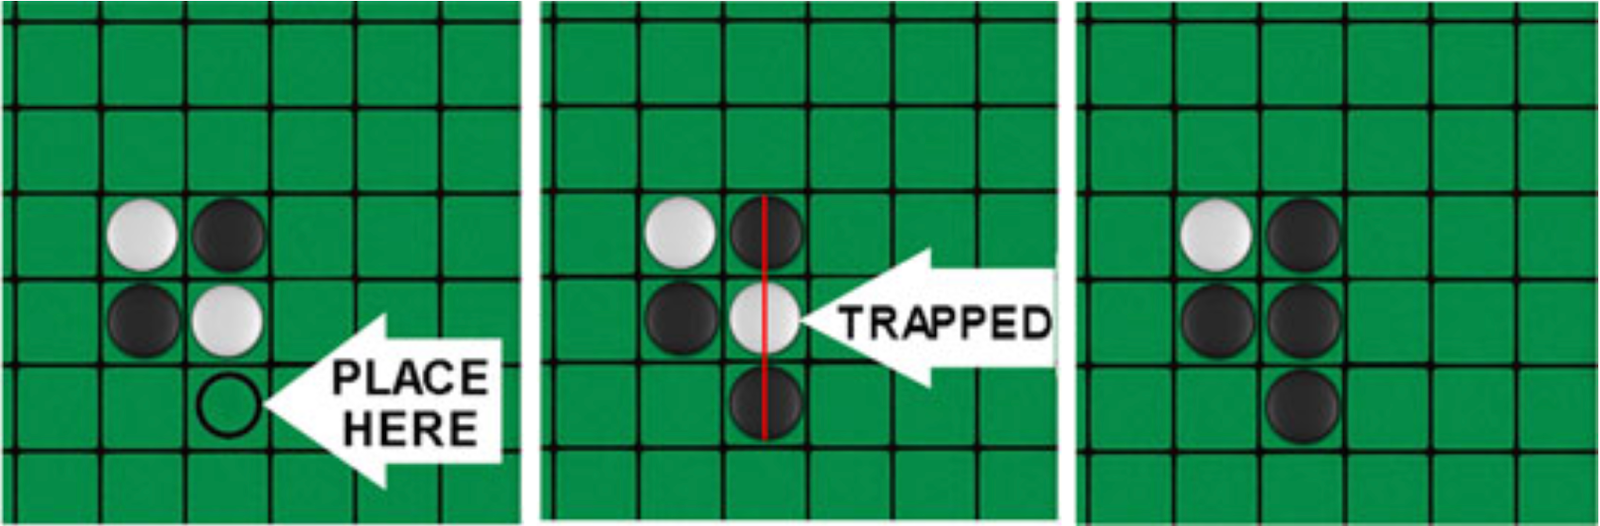
\includegraphics[width=0.75\linewidth]{figures/valid_move.png}
\caption{\label{fig:valid_move}Example of a valid move. Taken from: \cite{picture}}
\end{figure}
\\The example shows only one tile trapped between the dark discs, however this can be extended so that several tiles are trapped between one players pieces. In this instance, all of the trapped tiles are flipped before the next player is able to make their move.

\subsection{\label{doc:env_desc}Environment Description}

The design of our environment takes into account a number of common pieces: the state space, the set of actions, and the transition function. There are also a number of situationally dependent portions: the reward, the utility, the policy, and the value function. The state is easily represented as the current state of the board, which considers the number of opposing discs, the number of our own discs, and the positions of each disc. The set of actions is a layer which is the size of the Othello board where we simply apply a mask of the list of legal moves at the current state. The transition function is a deterministic function which indicates which discs will be flipped once an action has been played. The reward function for the positional agent is adapted slightly from the van Eck and van Wezel paper, and is given as the difference between the number of discs owned by player 1 minus those of player 2 if the game is in an end state, or 0 if we are not in an end state. We also implement a random starting strategy for the first three moves of the game. This was added to the learning agent to visit more possible game states to improve robustness when playing against different players. During the learning phase we implement an \textit{Epsilon Greedy} policy to make the next move with an exponential decay rate starting after the learning warm up phase. 
% Since these are the only options considered by their models, the utility function is irrelevant to the decision making process in the learning phase \cite{vanEck2008}.

\subsection{\label{doc:env_agnts}Environment Agents}
We are using an environment for the Othello game \cite{codes}, containing one positional and eight different AI algorithms playing Othello:
\begin{itemize} 
    \item EvalBoard \textit{(positional player)}:   Returns the action giving the best next state, according to the EvalBoard() function (see section \ref{doc:env_func})
    \item Minimax:   Minimising the maximum loss, a.k.a. maximising the minimum reward.
    \item Minimax w/ Alpha-Beta Pruning:    Aims to decrease the number of potential moves evaluated
    \item Negamax:  Version of Minimax, utilising the fact that:
    \begin{equation*}
        Value(board, player 1) = -Value(board, player 2)
    \end{equation*}
    \item Negamax w/ Alpha-Beta Pruning
    \item Negascout (Principal Variation Search):  Extension of Negamax which aims to be faster than Negamax with Alpha-Beta Pruning by never considering nodes which wouldn’t be considered by Alpha-Beta Pruning and further reducing the search space.
    \item Minimax w/ Alpha-Beta Pruning w/ Sorted Nodes:    Prioritising high-valued moves when searching by making use of the GetSortedNodes() function (see section \ref{doc:env_func}).
    \item Negamax w/ Alpha-Beta Pruning w/ Sorted Nodes
    \item Negascout (Principal Variation Search) w/ Sorted Nodes 
\end{itemize}

\subsection{\label{doc:env_func}Environment Functions}
The environment provides us with a few native functions that we take advantage of when implementing our playing agent\cite{codes}. The environment has been converted into a \texttt{Board} class which maintains the current state of the game and handles all of the functions below.
\begin{itemize}
    \item \texttt{InitBoard()}: Initialises the board in Othello starting position.
    \item \texttt{PrintBoard()}: Prints the current state of the board.
    \item \texttt{MakeMove()}: Assuming a valid move is provided, the agent makes the move at the specified position. Returns the board in its updated state and the count of how many tiles were flipped in the move-makers favour.
    \item \texttt{ValidMove()}: Checks if the move provided is valid. Returns boolean result
    \item \texttt{EvalBoard()}: Naively calculates the value of the board assuming corners are worth 4 points, edges are worth 2 points, and interior cells are worth one point. The function returns the total board score. In our \texttt{Board} class this function is called: \texttt{their\_eval\_board()}
    \item \texttt{IsTerminalNode()}: If there are no valid moves, the function returns true and marks the end of the game.
    \item \texttt{GetSortedNodes()}: Plays all possible moves for the agent and calculates the value of the board for each such move. Then the results are sorted in decreasing order: Highest valued moves first.
    \item \texttt{BestMove()}: Returns the best move according to the indicated playing agent.
\end{itemize}
We added a few functions to the environment which were necessary for the training phase described in section \ref{doc:train_phase}.
\begin{itemize}
    \item \texttt{set\_board()}: Sets \texttt{Board.board} to the passed in board state.
    \item \texttt{board\_to\_numpy()}: Converts user friendly appearance board to numpy board.
    \item \texttt{count\_board()}: Counts the number of discs the provided player has.
    \item \texttt{our\_EvalBoard()}: Evaluates the value of a position given a certain value function, like the one presented in section \ref{doc:positional}.
\end{itemize}

\section{Description of the algorithms}
For our experiments, we planned to implement the Q-learning algorithm, as specified in section 2.1 of \cite{vanEck2008}:

\begin{figure}[ht]
    \centering
    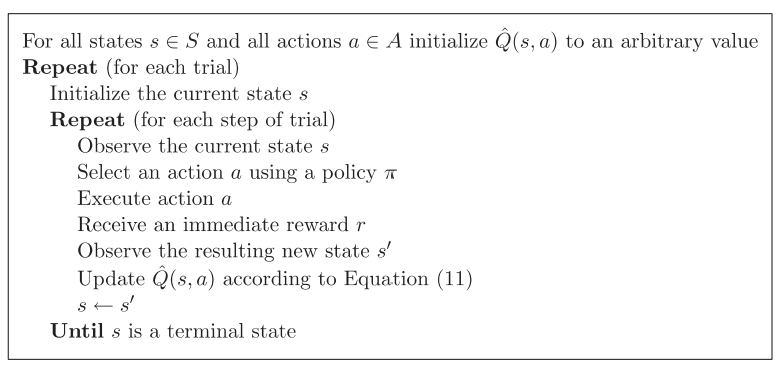
\includegraphics[width=0.9\linewidth]{figures/Q_algo.png}
    \caption{\label{fig:Q_algo}Pseudo-code for Q-Learning algorithm}
\end{figure}

\noindent Where Equation (11) is:

\begin{equation}
    \hat{Q}(s, a) \leftarrow (1-\alpha)\hat{Q}(s,a) + \alpha\left(r+\gamma \text{max}_{a'\in A}\hat{Q}(s', a')\right)
\end{equation}
\\
However, Othello has a massive state space, which means that something needs to be done to address this. One such approach is the class of function approximators. In section 2.1 of van Eck and van Wezel \cite{vanEck2008}, they outline an algorithm whose pseudo code can be seen here in figure \ref{fig:deep_Q_algo}.

\begin{figure}[ht]
    \centering
    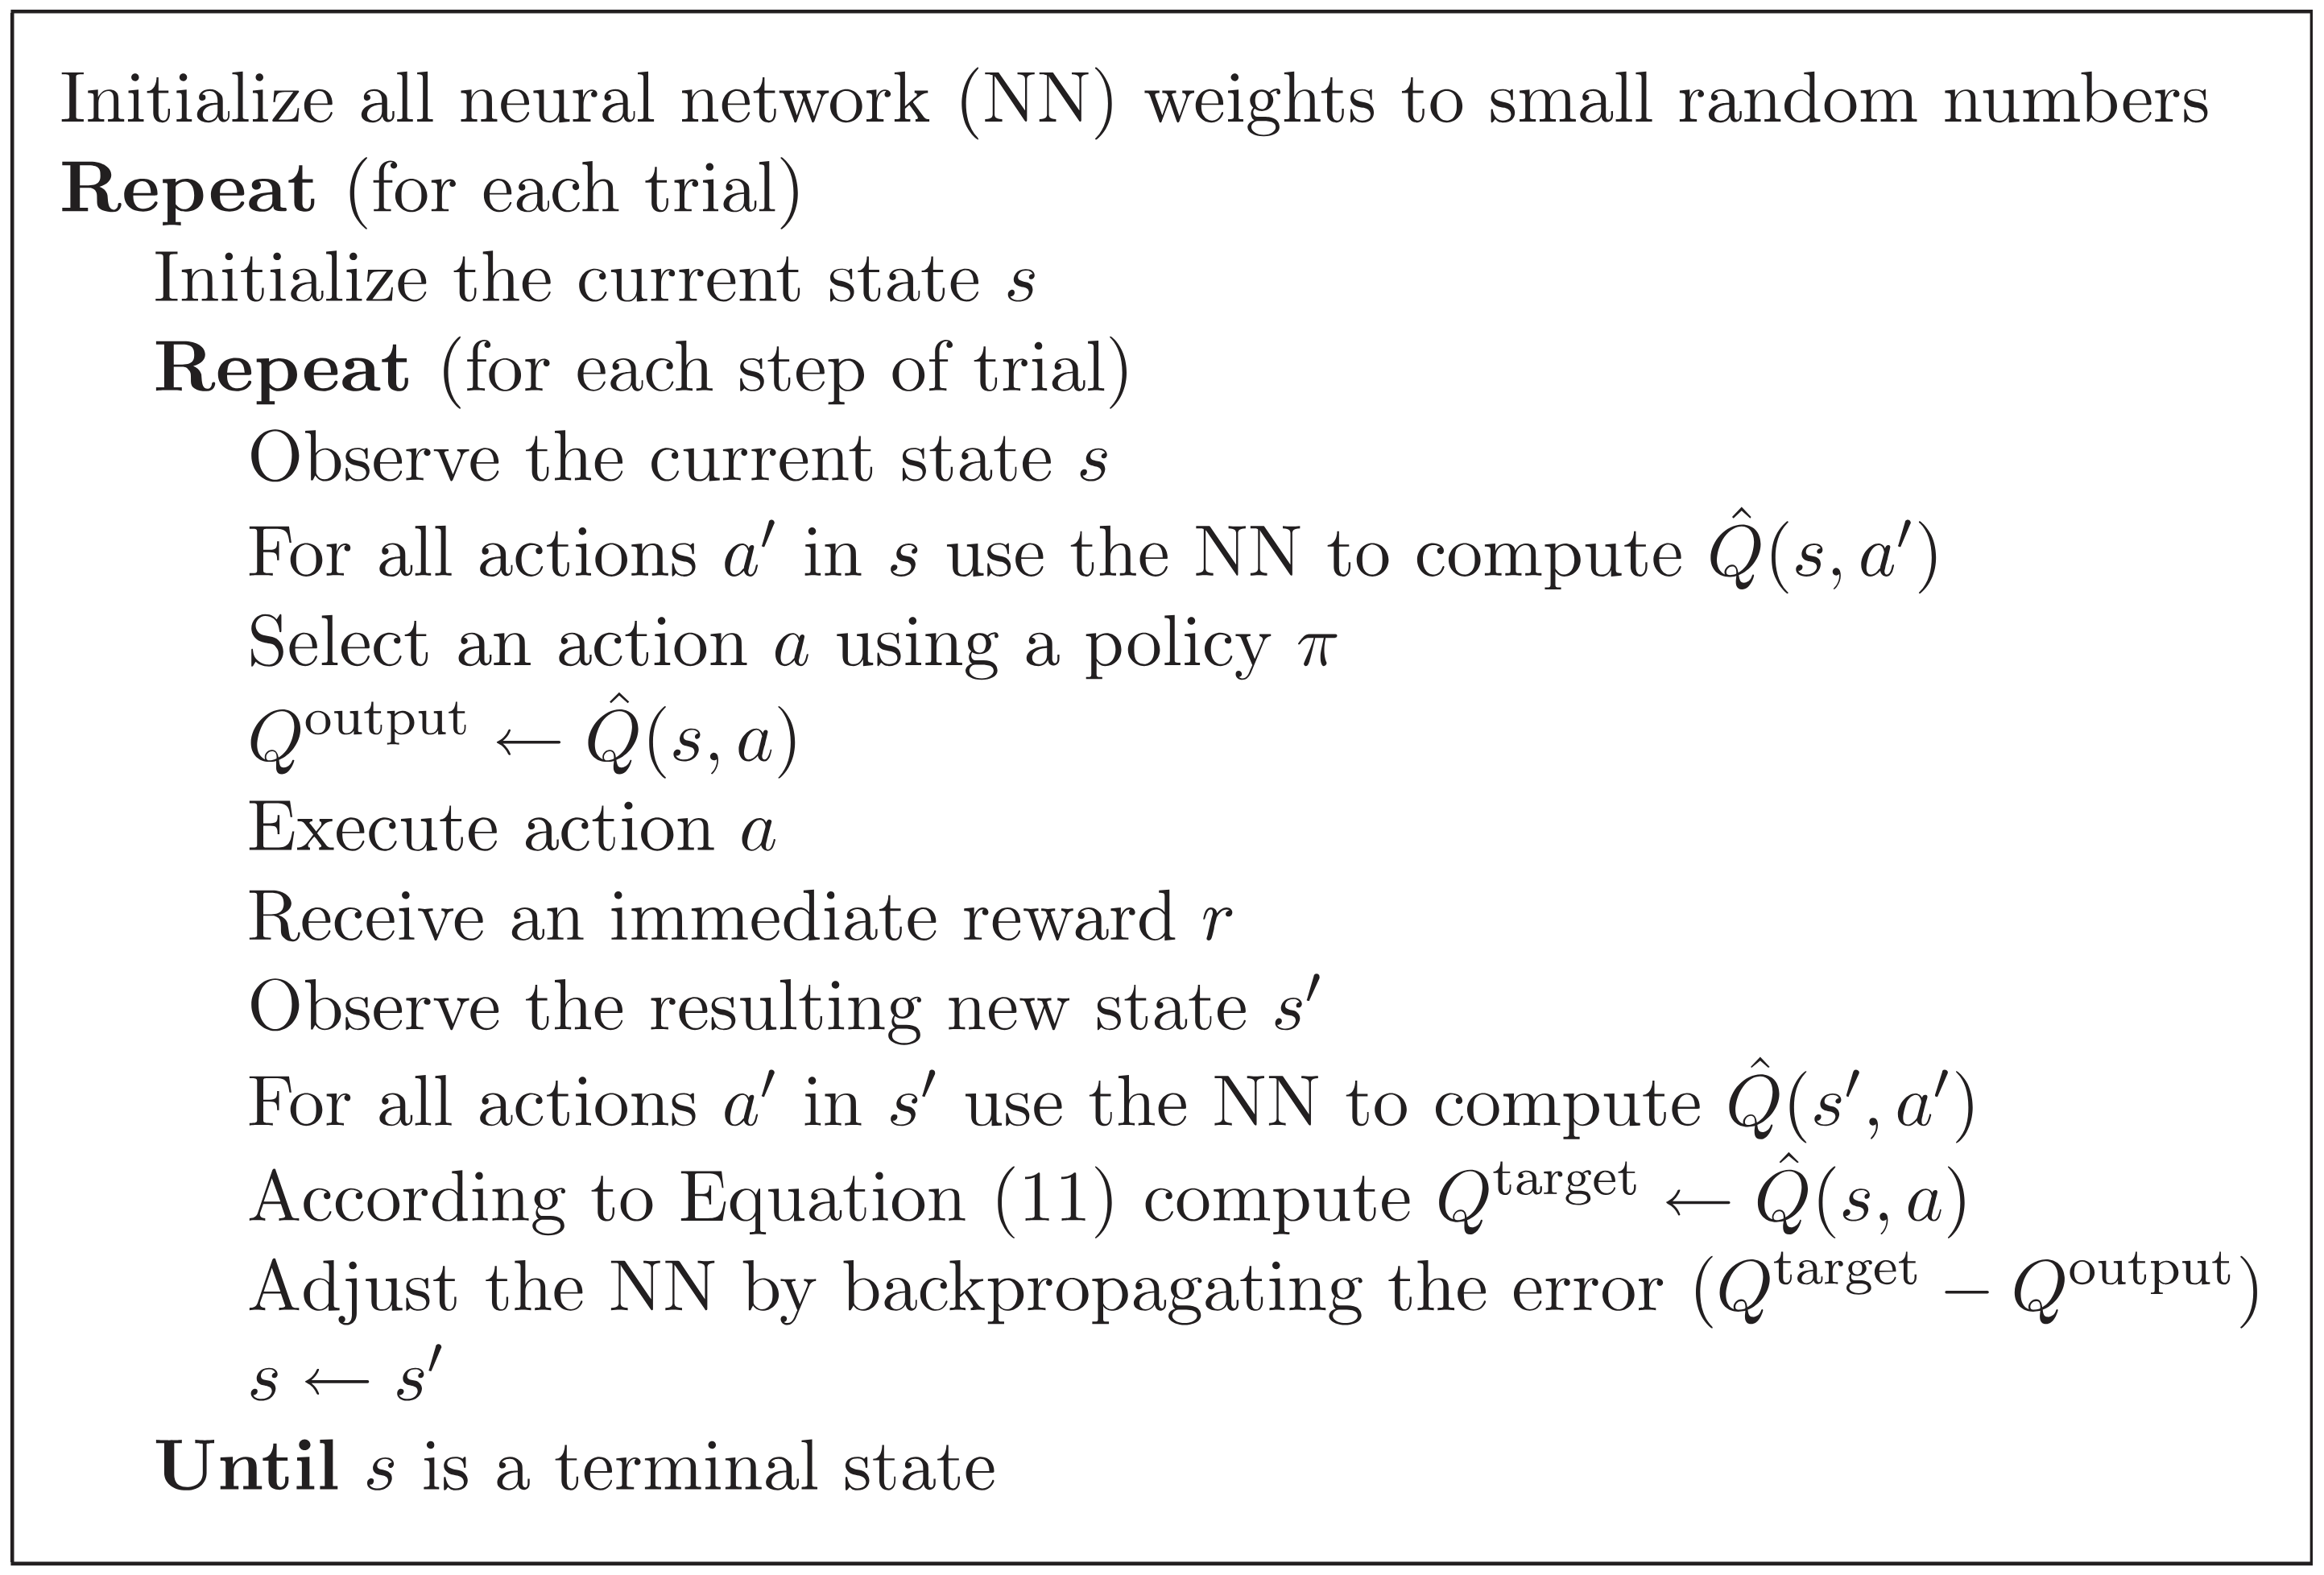
\includegraphics[width=0.9\linewidth]{figures/Deep_Q_Algo.png}
    \caption{\label{fig:deep_Q_algo}``The $Q$-learning algorithm with a feedforward neural network as function approximator" \cite{vanEck2008}}
\end{figure}

\noindent
For an explanation of the models designed for our experiments, please reference section \ref{doc:q_net}. The action is then chosen based on a weighted probability which considers the benefit of exploiting our current knowledge or exploring a new action to gain more knowledge of different moves. We can decrease the exploration rate over time, so that as we gain more information, we are more likely to exploit what we know rather than to explore different actions.
\\\\
In our case, we define two Neural Networks (NN), a \textit{target} network and an \textit{output} network. The \textit{target} network maintains the current ``best" approximation of the network and the \textit{output} network is the on-policy network which is updated throughout the training process. The training cycle of our project closely follows the \textit{Deep Q-Learning} script provided to us in the class \cite{DQN} which bears resemblance to the algorithm proposed in figure \ref{fig:deep_Q_algo}

\subsection{\label{doc:pol}Policy}
For both the self-play \ref{doc:self_play} and positional \ref{doc:positional} learned models, we implemented an \textit{Epsilon Greedy} action policy as described in \cite{RL_book}. 
\\\\
For both models, we input the state of the game into the learning network for the forward pass and apply a legal action filter to consider only legal actions in the given state. We then take the \textit{argmax} over the actions of the output and choose between this value and a random action from the list of legal actions with probability $\left[1-\epsilon, \epsilon\right]$.
\\\\
So, with the estimated best action $\mathcal{A}^*\overset{\Delta}{=} arg\underset{a}{max}\  \hat{Q}(s,a)$ and $\mathcal{A}$ being defined as the uniform distribution of all other actions, our policy is given by
$$
\hat{\pi}_{\epsilon}^* \overset{\Delta}{=} (1-\epsilon)\mathcal{A}^* + \epsilon \mathcal{A}
$$
where $\epsilon$ denotes the exploration rate, deciding to which degree we should explore other actions than the one we assume to be the best.

\subsection{\label{doc:q_net}$Q$-Network Design}
Akin to the NN design in \cite{vanEck2008}, we have an single hidden layer NN with both an input layer and an output layer of size 64x1. The state of the board is passed into the neural network where empty spaces take the value 0, spaces occupied by player 1 take the value 1, and spaces occupied by player 2 take the value 2. The hidden layer has 128 neurons, we did not try to optimize the size of the hidden layer as training times were longer than anticipated.

\subsection{\label{doc:train_phase}Training Phase}
Our training phase starts with a warm-up of 1000 games, where our transition buffer is fed with enough game states to initiate our \textit{target network} $Q^{target}$.
\\\\
Following the warm-up phase, the agent is trained by playing a certain number of games against a given opponent. After every game,  \textit{the agent's $Q$-network $\pi$} is updated by looking back on its actions, and comparing them to the target network.
\\\\
The computed loss (MSE) between the expected utility of our agent's actions and the ``true" $Q$-values sampled from our target, is used to update both $Q^{target}$ and $\pi$.
\\\\
The update of $\pi$'s parameters are handled by \texttt{torch.optim.Adam}, while the parameters of $Q^{target}$ are updated by
$$Q^{target} = (1-\tau)Q^{target} + \tau\pi,$$ where $\tau$ is the update value.
\\\\
Our \textit{Self-Play Agent} us trained by playing its own accumulated \textit{Q}-network, while the \textit{Positional Learning Agent} is trained by playing against the (non-learning) \textit{Positional Player}. These two agents are described in more detail in the following two subsections.


\subsection{\label{doc:self_play}$Q$-Network - Self-Play}
To avoid dealing with the uncertainty of playing an unknown opponent, we implemented a self-learning agent. Here we define two networks, a policy network and a target network. The policy network is our online learning agent and the target network is the agent which we use to approximate our network. Both the policy network and the target network have the same structure as defined in section \ref{doc:q_net}. We follow the training regiment defined in \ref{doc:train_phase} and our agent plays as player 1 against the target network. That is to say, for each state of the board, it is either player 1's move, or player 2's move. On player 1's move we take our action from the \textit{Epsilon Greedy} policy defined \ref{doc:pol}. Whereas, on player 2's move, we take our action from the target network's best move with no additional policy adjustments.


\subsection{\label{doc:positional}$Q$-Network - Positional Learning}
We also implemented a positional learning player, which learns similarly to the self-playing agent described above. In place of the target network making player 2's move, we have implemented a positional player which makes use of the position value matrix from \cite{vanEck2008} provided below in figure \ref{fig:pos_vals}.
\begin{figure}[ht]
\centering
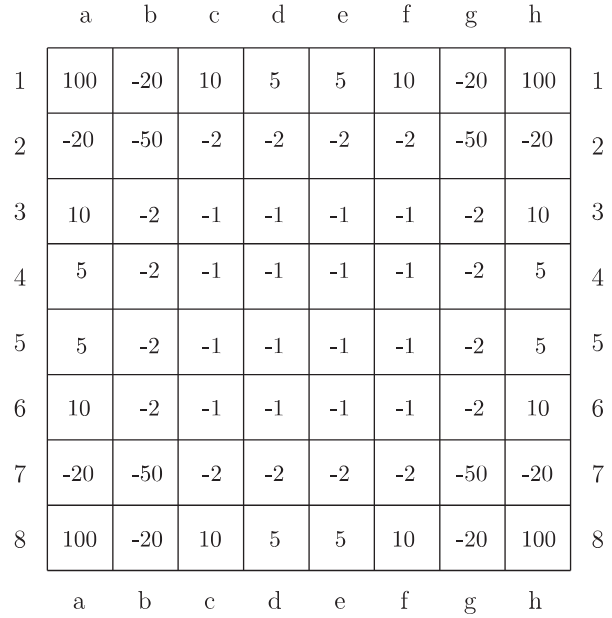
\includegraphics[width=0.6\linewidth]{figures/position_vals.png}
\caption{\label{fig:pos_vals}Position Value Matrix as outlined in \cite{vanEck2008}.}
\end{figure}
\\
This takes advantage of some expert knowledge which defines corner squares to be more valuable and positions which give away corner squares to be less valuable. We hypothesized that this would lead to our agent learning the game faster. This will be discussed further in \ref{doc:exp_results}

\section{\label{doc:exp_results}Experimental Results}
Unfortunately, the results of our experiments did not pan out the way we had expected them to. As detailed in the `Future work' section of our mid-term report, we implemented a 4x4 $Q$-learning agent which yielded a promising training curve as seen in figure \ref{fig:4x4_curve}.
\begin{figure}[ht]
\centering
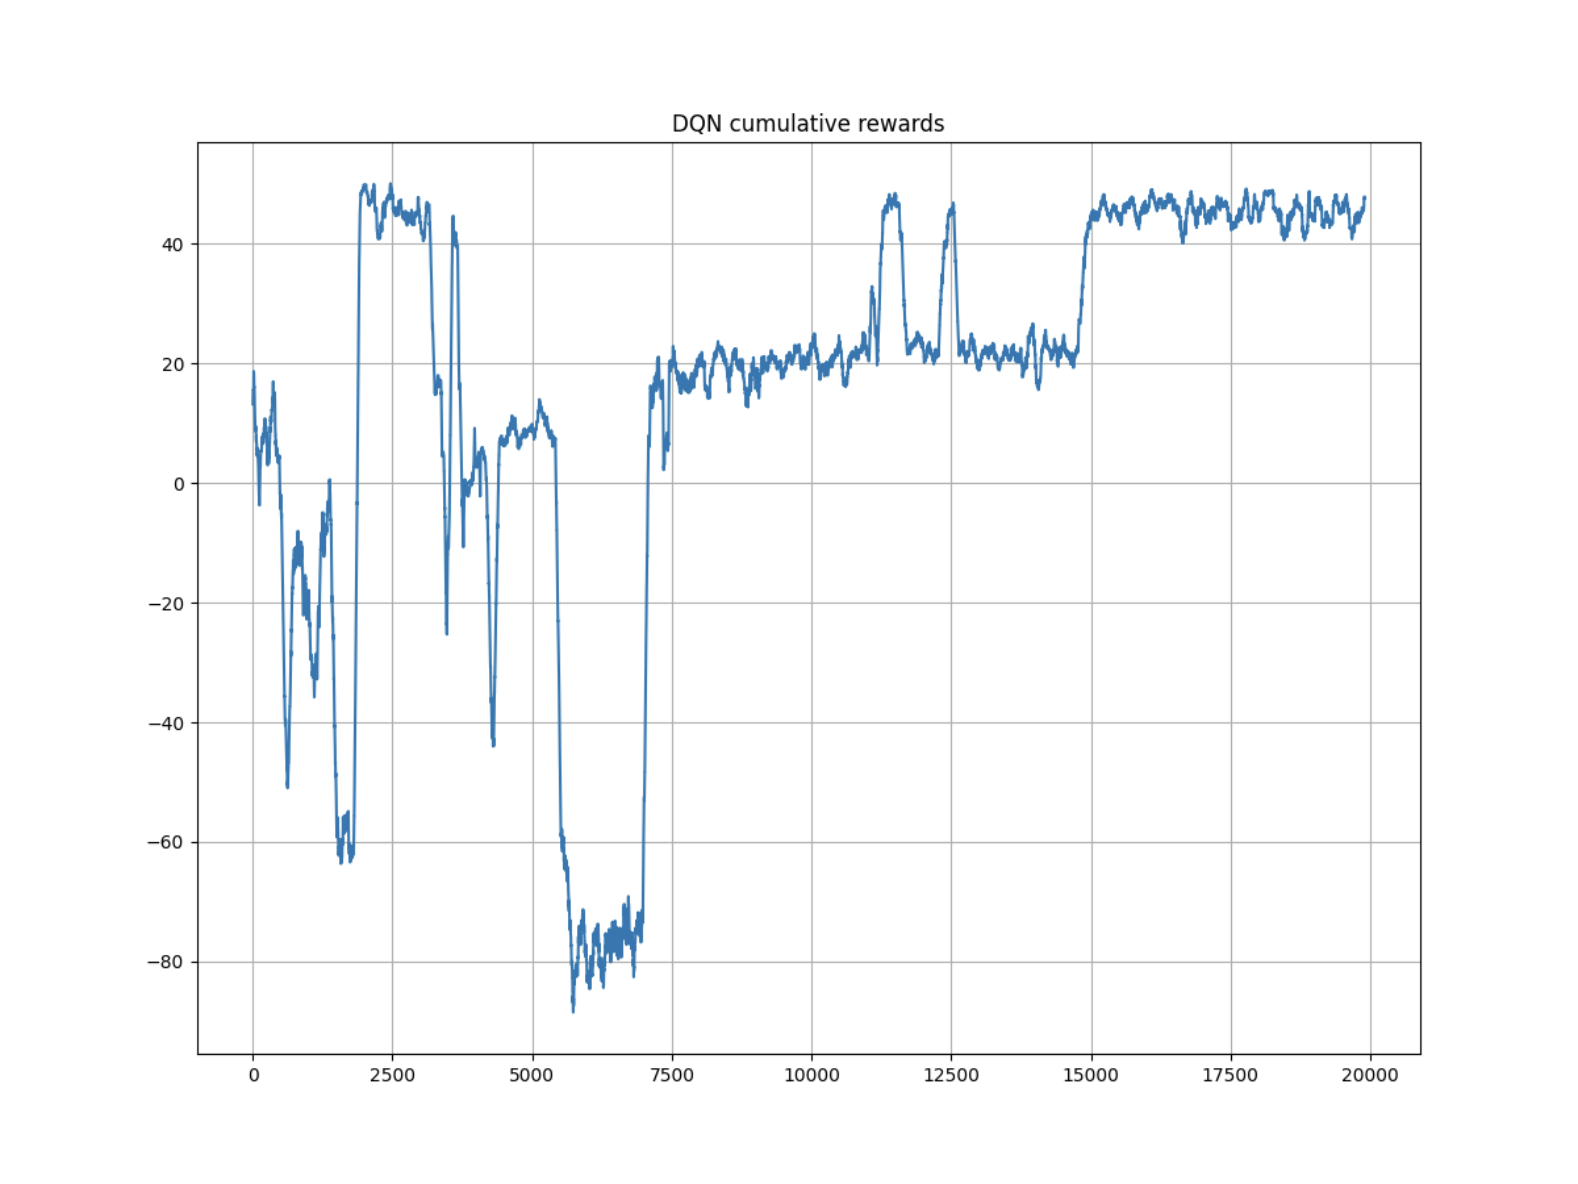
\includegraphics[width=0.9\linewidth]{figures/4x4_model_cumulative_rewards_curve.png}
\caption{\label{fig:4x4_curve}Running mean plot of a 4x4 learning curve.}
\end{figure}
This lead to another promising training curve as seen in figure \ref{fig:8x8_good_curve}.
\begin{figure}[ht]
    \centering
    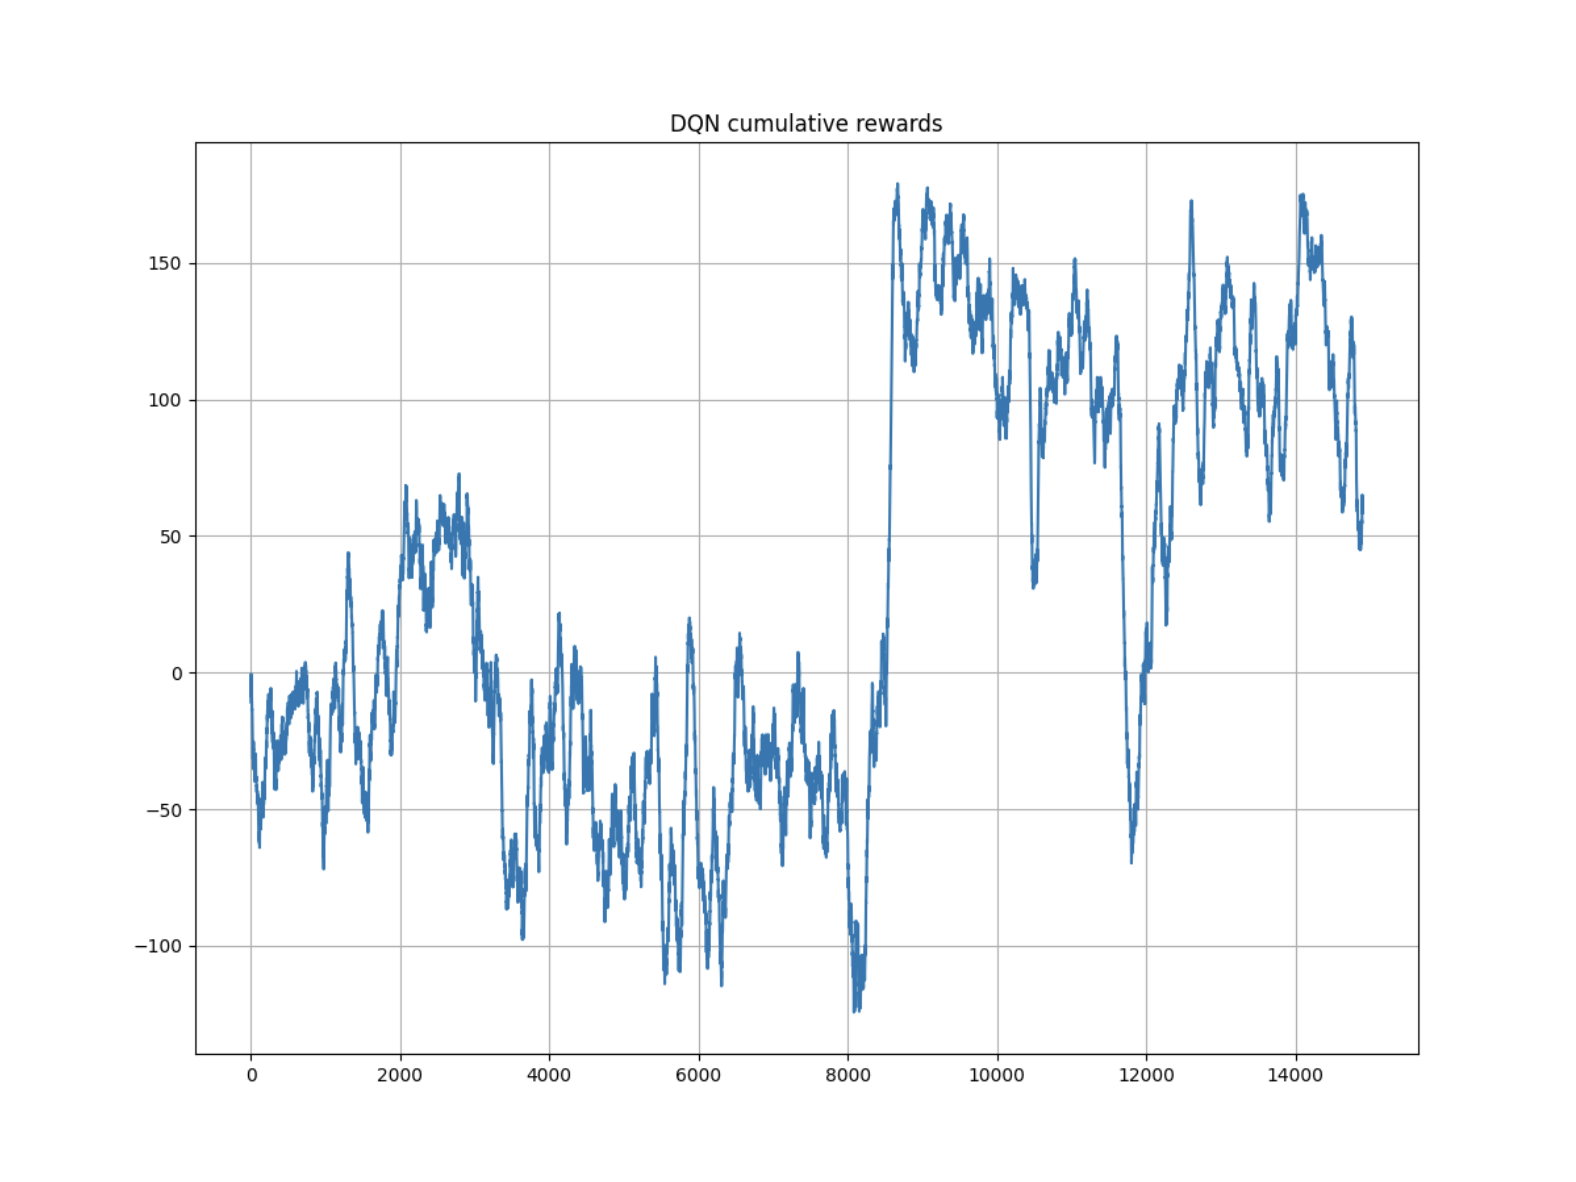
\includegraphics[width=0.9\linewidth]{figures/8x8_model_cumulative_reward_curve.png}
    \caption{\label{fig:8x8_good_curve}Running mean plot of an 8x8 learning curve.}
\end{figure}
\\\\
However, these promising results quickly ground to a halt upon the realization that the model was playing illegal moves and placing disks when searching for legal actions. This meant that the model would ``find" legal moves when there were none, which obviously tilts the board in their favor.
\\\\
After fixing this error, we found that the training had taken a turn towards the worst. Following dozens of retrainings, each taking up to three hours to complete, the model's training curves looked something like that in figure \ref{fig:8x8_current_curve}.
\begin{figure}[ht]
    \centering
    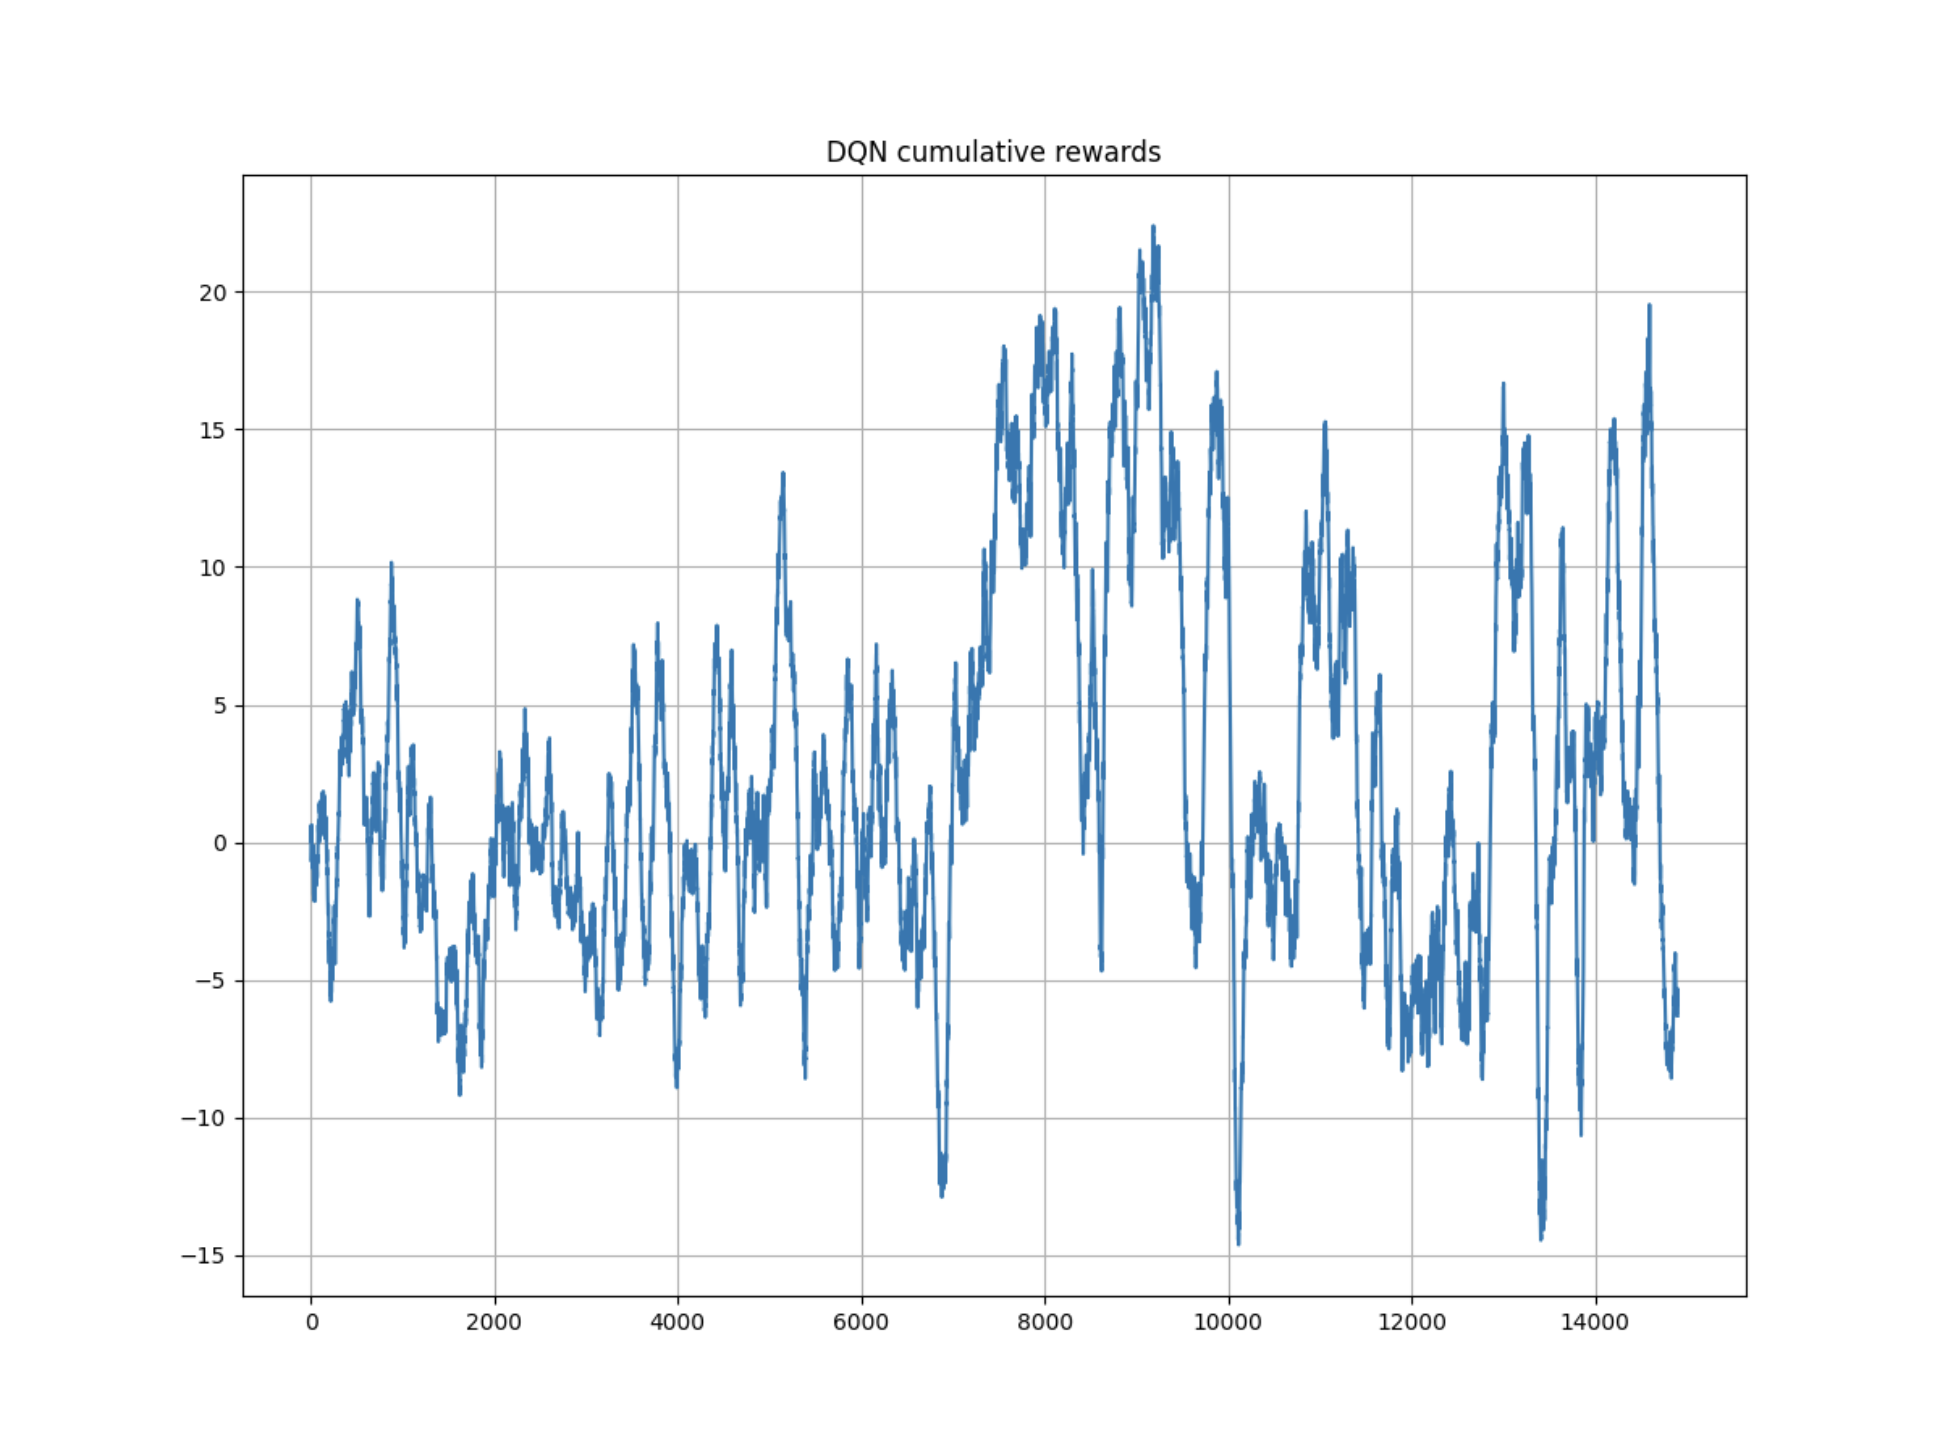
\includegraphics[width=0.9\linewidth]{figures/8x8_current_training_curve.png}
    \caption{\label{fig:8x8_current_curve}Current running mean plot of an 8x8 learning curve.}
\end{figure}
\\\\
We still tested these models against the two positional players as base-line quality metrics, here are the two winning proportion graphs in figure \ref{fig:winning_rates}. As we can see from the graph from \cite{codes}'s positional player, there does appear to be a slight up-trend throughout the course of training. We have concluded that the positional player presented in \cite{vanEck2008} is a significantly stronger player than the positional player from \cite{codes}. This notion is indeed confirmed in the two plots presented in figure \ref{fig:winning_rates}.

\begin{figure}[ht]
    \centering
        % \begin{subfigure}
    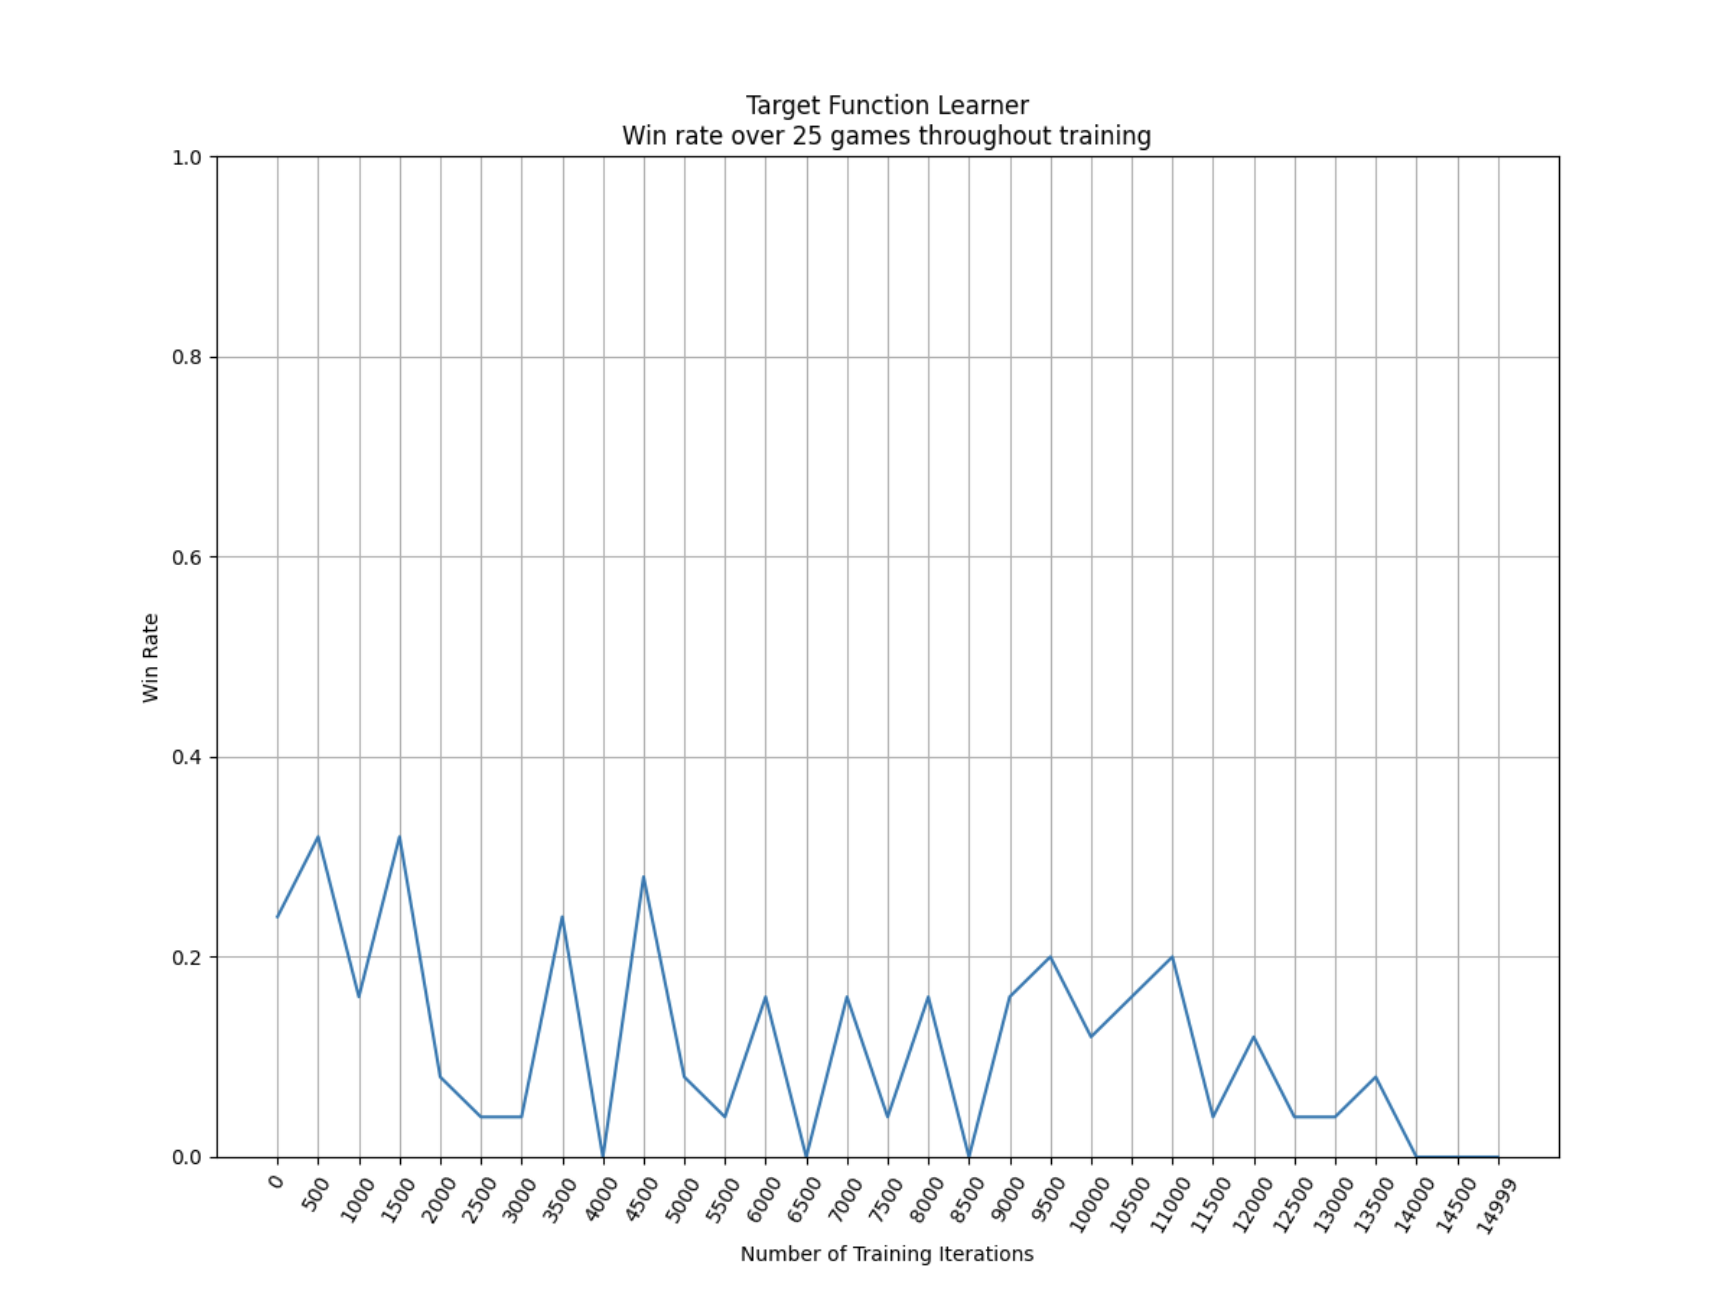
\includegraphics[width=0.99\linewidth]{figures/8x8_win_rate_our_positional_player.png}
    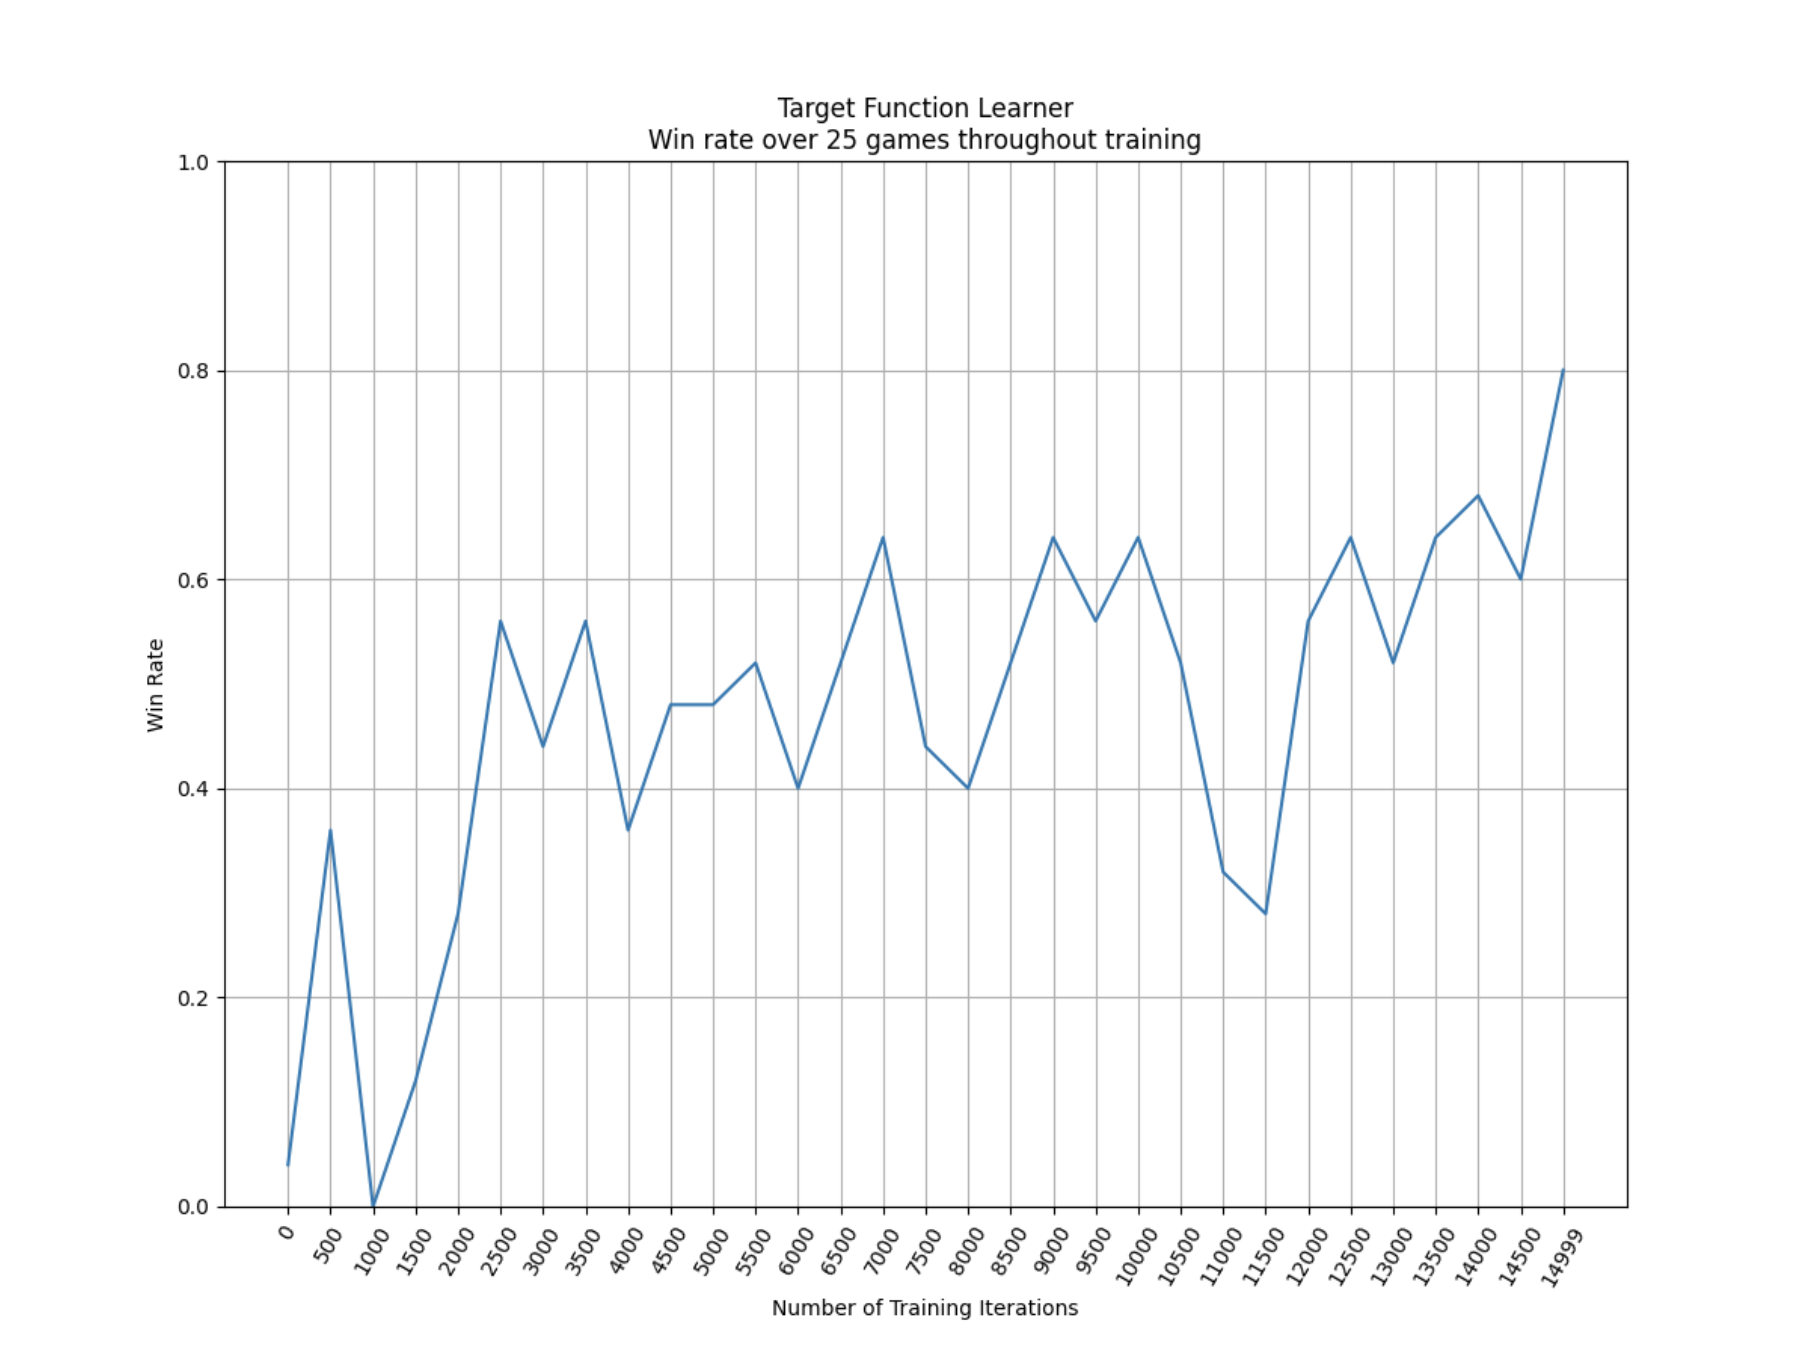
\includegraphics[width=0.99\linewidth]{figures/8x8_win_rate_their_positional_player.png}
        % \end{subfigure}
    \caption{\label{fig:winning_rates}Win-rate graphs, (upper) positional player from \cite{vanEck2008}, (lower) positional player from \cite{codes}}
\end{figure}

\section{Future work}
Based on our results, we believe that it would be beneficial to increase the number of training iterations. Looking at van Eck \& van Wezel's project, they trained their agents on 15,000,000 games, compared to our 15,000. So this would be a natural place to start to try to improve our results.
\\\\
Additionally, future experiments could involve tuning the hyperparameters in order to get a more accurate and stable model.
\\\\
Finally, we think testing different variations on the hidden layers -- both in size and in numbers -- could be an interesting follow-up of our work. 

\section{Conclusion}
As discussed in our future work section, there are a number of changes which we believe could bring some stronger results to our project. Despite the slight appearance of learning presented and discussed in figure \ref{fig:winning_rates}, it seems that our trained model is struggling to learn throughout the training phase. It suffices to say, that we would need to see the quality of a model with more training iterations before completely nixing the approach which we have taken. It is of course possible that there are some errors in our implementation, however it is often difficult to locate these small niggles in the code, especially after seeing a glimmer of hope. All in all, we have been able to produce an agent which learns with a function approximated $Q$-learning approach, albeit the resulting player is not as strong as we would like it to be.
\\
Our code base is accessible in \cite{our_code}.
\\\\\\\\\\\\\\\\\\\\\\\\\\\\\\\\\\\\
\printbibliography

\end{document}
